\documentclass{article}

\usepackage{graphicx}
\usepackage{tikz}
\usepackage{tikzsymbols}
\usetikzlibrary{calc,patterns,shapes.geometric}
\pagestyle{empty}
\usepackage[margin=0pt]{geometry}
\geometry{papersize={14in,12in}}

\def\centerarc[#1](#2)(#3:#4:#5){\draw[#1] ($(#2)+({#5*cos(#3)},{#5*sin(#3)})$) arc (#3:#4:#5);}

\begin{document}
	\begin{figure}
		\centering
		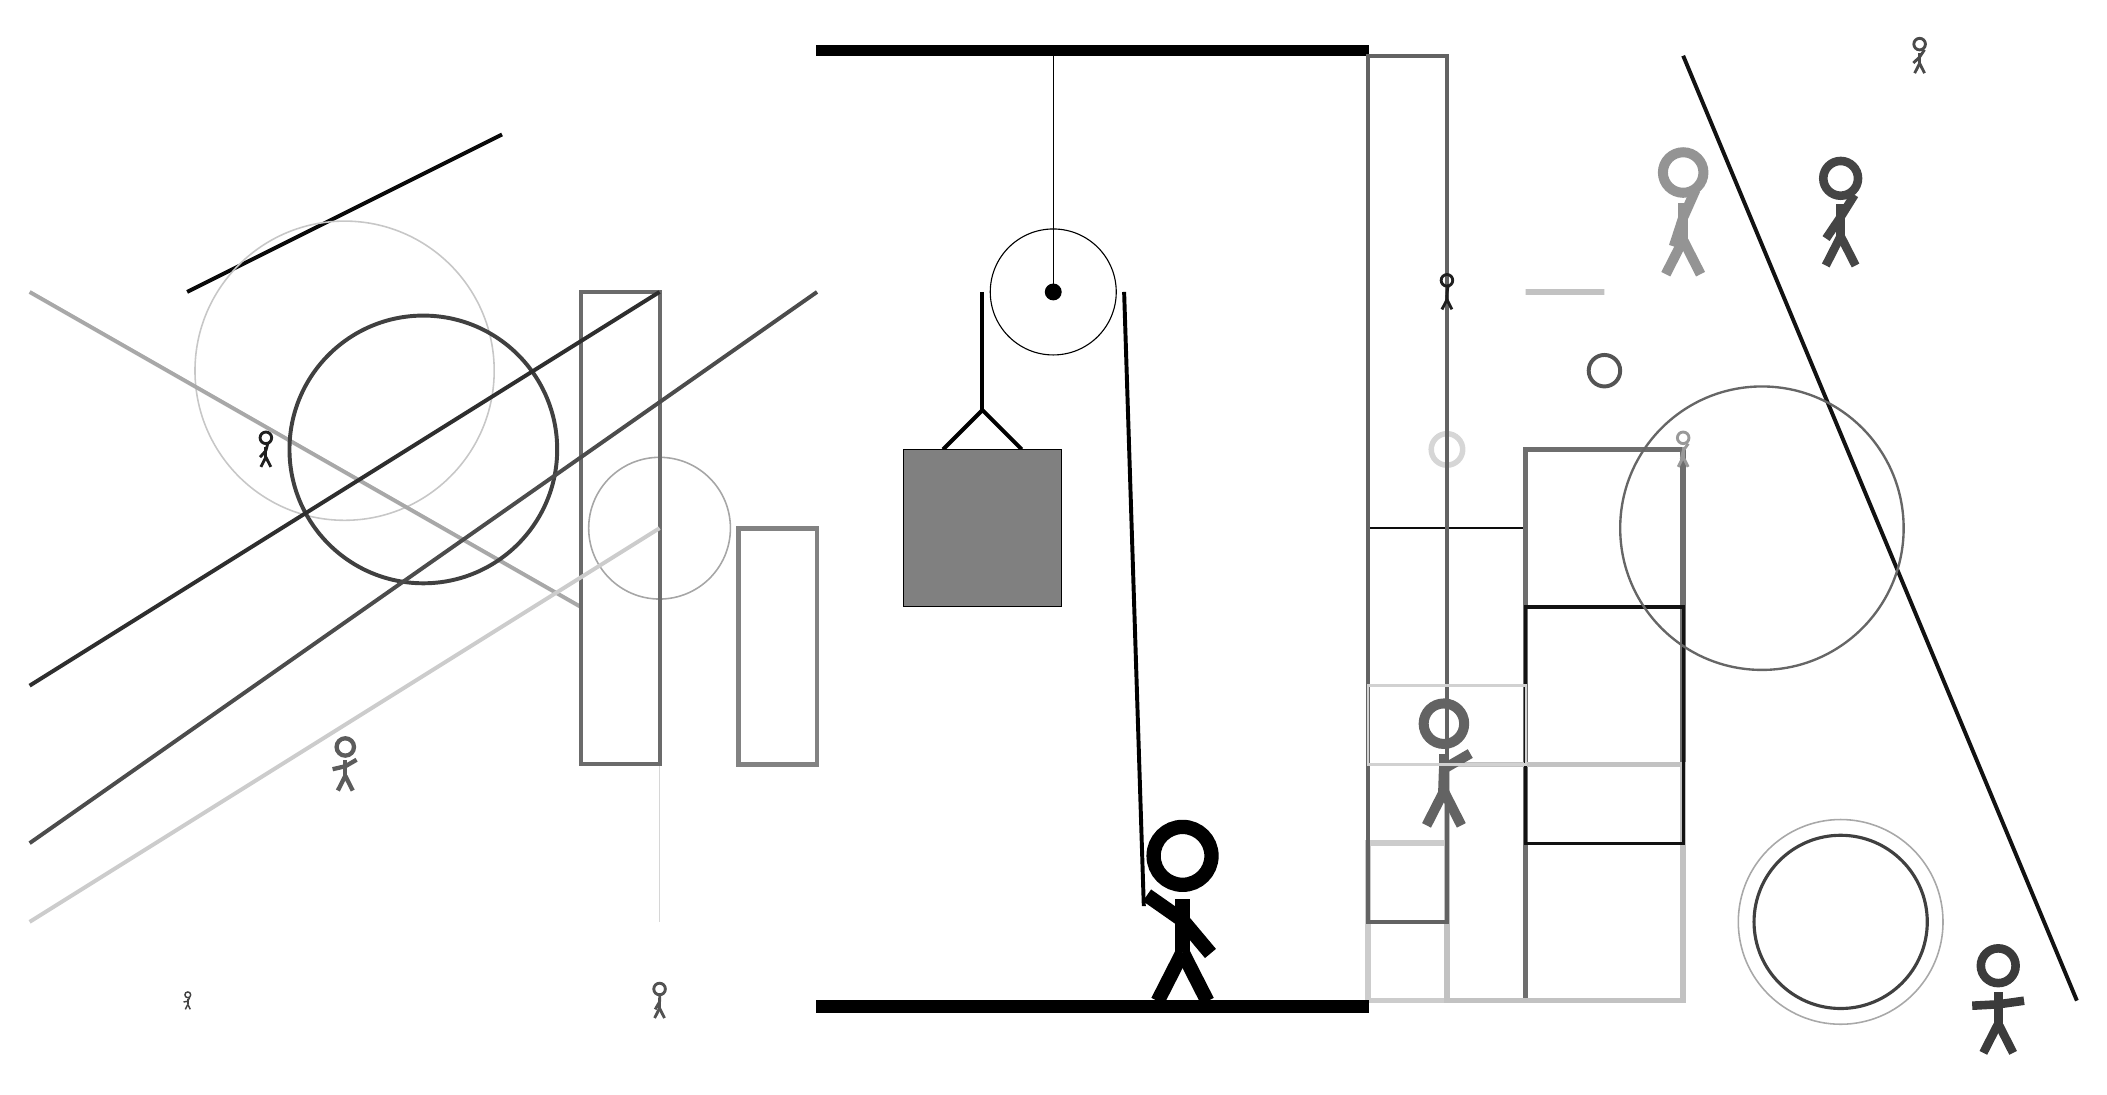
\begin{tikzpicture}
			%%%%% START %%%%%
			
			\draw[fill=black] (-2, 9) rectangle (5, 9.125);
			
			\draw (1, 6) circle (0.8);
			\draw[fill=black] (1, 6) circle (0.1);
			\draw (1, 9) -- (1, 6);
			
			\draw [line width=0.7mm, color=black!16](6, 4) circle (0.2);
			
			\draw[line width=0.5mm, color=black!96](-6, 8) -- (-10, 6);
			\draw[line width=0.2mm, color=black!95] (7, 3) rectangle (5, 3);
			\draw[line width=0.7mm, color=black!20] (6, -3) rectangle (5, -1);
			
			\draw[line width=0.2mm, color=black!16] (-4, 6) rectangle (-4, -2);
			\draw [line width=0.2mm, color=black!35](-4, 3) circle (0.9);
			\draw[line width=0.7mm, color=black!57] (7, -3) rectangle (9, 4);
			
			\node[line width=0.7mm, color=black!77] at (13, -3) {\Strichmaxerl[6][3][8]};
			\draw [line width=0.5mm, color=black!67](8, 5) circle (0.2);
			\draw[line width=0.7mm, color=black!24] (6, -3) rectangle (9, 0);
			
			\draw [line width=0.2mm, color=black!22](-8, 5) circle (1.9);
			\draw[line width=0.5mm, color=black!34](-5, 2) -- (-12, 6);
			\draw[line width=0.5mm, color=black!61] (6, -2) rectangle (5, 9);
			
			\draw [line width=0.4mm, color=black!75](11, -2) circle (1.1);
			\draw[line width=0.5mm, color=black!58] (-4, 6) rectangle (-5, 0);
			\draw[line width=0.5mm, color=black!93](9, 9) -- (14, -3);
			\draw [line width=0.2mm, color=black!34](11, -2) circle (1.3);
			\draw[line width=0.4mm, color=black!93] (7, 2) rectangle (9, -1);
			\node[line width=0.7mm, color=black!71] at (12, 9) {\Strichmaxerl[2][44][56]};
			\draw[line width=0.7mm, color=black!24] (7, 6) rectangle (8, 6);
			\draw [line width=0.5mm, color=black!75](-7, 4) circle (1.7);
			
			\node[line width=0.4mm, color=black!42] at (9, 7) {\Strichmaxerl[7][72][66]};
			
			\draw[line width=0.6mm, color=black!49] (-2, 0) rectangle (-3, 3);
			\node[line width=0.3mm, color=black!73] at (11, 7) {\Strichmaxerl[6][56][58]};
			\node[line width=0.2mm, color=black!64] at (-8, 0) {\Strichmaxerl[3][13][30]};
			
			\node[line width=0.4mm, color=black!68] at (-4, -3) {\Strichmaxerl[2][60][88]};
			
			\node[line width=0.5mm, color=black!61] at (6, 0) {\Strichmaxerl[7][88][30]};
			\node[line width=0.7mm, color=black!88] at (6, 6) {\Strichmaxerl[2][89][81]};
			\node[line width=0.3mm, color=black!88] at (-9, 4) {\Strichmaxerl[2][48][75]};
			\node[line width=0.2mm, color=black!40] at (9, 4) {\Strichmaxerl[2][77][54]};
			\draw[line width=0.5mm, color=black!20](-4, 3) -- (-12, -2);
			
			\draw[line width=0.3mm, color=black!18] (5, 1) rectangle (7, 0);
			\draw[line width=0.5mm, color=black!70](-2, 6) -- (-12, -1);
			
			\draw[line width=0.5mm, color=black!82](-4, 6) -- (-12, 1);
			\node[line width=0.7mm, color=black!74] at (-10, -3) {\Strichmaxerl[1][10][65]};
			\draw [line width=0.3mm, color=black!60](10, 3) circle (1.8);
			
			\draw[line width=0.5mm] (-0.4, 4.0) -- (0.1, 4.5) -- (0.6, 4.0);
			\draw[fill=black!50] (-0.9, 4.0) rectangle (1.1, 2.0);
			
			\draw[line width=0.5mm] (0.1, 6) -- (0.1, 4.5);
			\centerarc[line width=0.5mm](1, 6)(0:180:0.9);
			\draw[line width=0.5mm](1.9, 6) -- (2.15, -1.8);
			
			\node at (2.6, -1.9) {\Strichmaxerl[10][-35][-50]};
			
			\draw[fill=black] (-2, -3) rectangle (5, -3.15);
			
			%%%%% END %%%%%
		\end{tikzpicture}
	\end{figure}	
\end{document}